\documentclass[a4paper,12pt]{article}
\usepackage[utf8]{inputenc}
\usepackage{graphicx}
\usepackage{url}
\usepackage{amsmath}
\usepackage{amssymb}
\usepackage{geometry}
\usepackage{booktabs}
\usepackage{pgfplotstable}
\usepackage{float}
\pgfplotsset{compat=1.18}
\geometry{
    a4paper,
    left=2.54cm,
    right=2.54cm,
    top=2.54cm,
    bottom=2.54cm,
}

\title{Estudio de la Ecuación de Schrödinger en Diferentes Pozos de Potencial}
\author{César de la Rosa Sobrino}
\date{\today}

\begin{document}

\maketitle

\begin{abstract}
  Este documento presenta un estudio numérico de la ecuación de Schrödinger independiente del tiempo para distintos pozos de potencial. Se emplean métodos numéricos basados en diferencias finitas y la integración numérica para discretizar la ecuación, permitiendo resolver el problema de autovalores para los niveles de energía y funciones de onda correspondientes.
\end{abstract}

\section*{Declaración de Autoría}

El trabajo presentado ha sido íntegramente realizado por el autor firmante, tanto en la generación de los resultados, como en su presentación y redacción de la memoria. Todos los códigos de programación han sido escritos por el autor o parten de los suministrados en la propia tarea práctica. Cualquier idea tomada de otros autores o fuentes externas ha sido debidamente citada y puede ser consultada por el lector del trabajo. Si se demostrara lo contrario, el abajo firmante aceptará las medidas disciplinarias o sancionadoras que correspondan.

\section*{Estimación de Horas Empleadas}

\begin{itemize}
    \item Horas de estudio del problema: 2,5 horas
    \item Horas de trabajo computacional: 5 horas
    \item Horas de redacción de la memoria: 6 horas
\end{itemize}
\section{Introducción}
La mecánica cuántica es una de las teorías fundamentales de la física moderna, describiendo el comportamiento de partículas a escalas microscópicas. Central en esta teoría es la ecuación de Schrödinger, que determina la evolución temporal y espacial del estado cuántico de un sistema. Este trabajo se enfoca en la resolución numérica de la ecuación de Schrödinger para diferentes tipos de pozos de potencial, permitiendo el análisis de sistemas donde las soluciones analíticas son inalcanzables.

\section{Fundamentos Teóricos}
En esta sección se abordan los conceptos clave de la mecánica cuántica necesarios para la resolución numérica de la ecuación de Schrödinger.

\subsection{Valores Esperados e Incertidumbres}
El valor esperado de un operador, como la posición $\hat{x}$ o el momento lineal $\hat{p}$, sobre una función de onda $\Psi(x)$ se define mediante:
\[
\langle O \rangle = \int_{-\infty}^{\infty} \Psi^*(x) \, O \, \Psi(x) \, dx
\]
Específicamente, para la posición y el momento:
\[
\langle x \rangle = \int_{-\infty}^{\infty} x |\Psi(x)|^2 \, dx, \quad \langle p \rangle = \int_{-\infty}^{\infty} \Psi^*(x) \left( -i\hbar \frac{\partial}{\partial x} \right) \Psi(x) \, dx
\]
Las incertidumbres $\Delta x$ y $\Delta p$ se calculan como:
\[
\Delta x = \sqrt{\langle x^2 \rangle - \langle x \rangle^2}, \quad \Delta p = \sqrt{\langle p^2 \rangle - \langle p \rangle^2}
\]
El principio de incertidumbre de Heisenberg establece que:
\[
\Delta x \Delta p \geq \frac{\hbar}{2}
\]

\subsection{Operadores y Hamiltoniano}
El operador de energía cinética está dado por:
\[
\hat{T} = -\frac{\hbar^2}{2m} \frac{\partial^2}{\partial x^2}
\]
El operador Hamiltoniano, que representa la energía total del sistema, se define como:
\[
\hat{H} = \hat{T} + \hat{V} = -\frac{\hbar^2}{2m} \frac{\partial^2}{\partial x^2} + U(x)
\]
La ecuación de Schrödinger independiente del tiempo es:
\[
\hat{H} \Psi(x) = E \Psi(x)
\]

\subsection{Métodos Numéricos}
Para resolver la ecuación de Schrödinger numéricamente, se emplean varias técnicas:

\subsubsection{Diferencias Finitas}
Se discretiza el dominio espacial en una malla de puntos $x_i = x_0 + i h$, y se aproximan las derivadas mediante diferencias finitas centradas:
\[
\frac{d\Psi(x)}{dx} \approx \frac{\Psi(x+h) - \Psi(x-h)}{2h}, \quad \frac{d^2 \Psi(x)}{dx^2} \approx \frac{\Psi(x+h) - 2\Psi(x) + \Psi(x-h)}{h^2}
\]
Esto transforma la ecuación en un sistema de ecuaciones lineales que puede resolverse eficientemente.

\subsubsection{Integración}
La integral para los valores esperados se aproxima utilizando la regla del trapecio:
\[
\int_a^b f(x) \, dx \approx \frac{h}{2} \left[ f(x_0) + 2 \sum_{i=1}^{n-1} f(x_i) + f(x_n) \right]
\]
\subsubsection{Normalización}
La función de onda se normaliza dividiendo por la raíz cuadrada de la integral:
\[
\Psi_{\text{normalizada}}(x_i) = \frac{\Psi(x_i)}{\sqrt{\sum_{i=1}^{n} |\Psi(x_i)|^2 \, h}}
\]


\section{Tipos de Pozos de Potencial}
Estudiaremos varios tipos de pozos de potencial, valorando su importancia como modelos de sistemas físicos distintos y entendiendo sus propiedades al variar distintos parámetros. De esta manera estudiaremos en primer lugar el potencial armónico y como una versión más compleja el potencial de dos pozos cercanos. A su vez, en segundo lugar estudiaremos el pozo de potencial finito para luego visualizar el modelo de Kronig-Penney como una función periódica de pozos de potencial finito

\subsection{Potencial Armónico}

El potencial armónico es uno de los modelos más fundamentales y estudiados en la mecánica cuántica. Se describe por la ecuación:

\begin{equation}
    U(x) = \frac{1}{2} m \omega^2 x^2
\end{equation}

donde \( m \) es la masa de la partícula y \( \omega \) es la frecuencia angular del sistema. Este potencial modela sistemas físicos como osciladores armónicos cuánticos, vibraciones moleculares y modos de vibración en sólidos.

Las soluciones de la ecuación de Schrödinger independiente del tiempo para este potencial son las funciones de Hermite \( \psi_n(x) \), que forman una base ortonormal en el espacio de funciones de onda. Los niveles de energía están cuantizados de forma equiespaciada y se expresan como:

\begin{equation}
    E_n = \hbar \omega \left(n + \frac{1}{2}\right)
\end{equation}

donde \( n \) es el número cuántico principal (\( n = 0, 1, 2, \ldots \)) y \( \hbar \) es la constante de Planck reducida. El término \( \frac{1}{2} \hbar \omega \) representa la energía de punto cero, indicando que el oscilador armónico no puede estar completamente en reposo incluso en su estado fundamental.

Este modelo es clave para entender cómo las partículas vibran alrededor de una posición de equilibrio, similar a los átomos en un enlace molecular. Además, el potencial armónico sirve como una aproximación válida para sistemas más complejos cerca de sus puntos de equilibrio, lo que facilita el análisis de fenómenos como las transiciones vibracionales y la espectroscopía molecular.

\begin{figure}[H]
    \centering
    \includegraphics[width=0.9\textwidth]{img/Potencial_Armónico.png}
    \caption{Potencial Armónico}
    \label{fig:potencial_armonico}
\end{figure}

\noindent
En la Figura \ref{fig:potencial_armonico} se observa el potencial armónico \( U(x) \) junto con los primeros diez niveles de energía \( E_n \) y sus correspondientes funciones de onda \( \psi_n(x) \). Cada nivel de energía está representado por una línea horizontal, reflejando la cuantización equiespaciada. Las funciones de onda, que son soluciones de la ecuación de Schrödinger, muestran diferentes formas dependiendo del número cuántico \( n \). En el estado fundamental, la función de onda es una distribución gaussiana simétrica alrededor del mínimo del potencial. A medida que aumenta \( n \), las funciones de onda exhiben más nodos, lo que indica niveles de excitación superiores.

\subsection{Potencial de Dos Pozos Cercanos}

El siguiente paso en complejidad respecto al potencial armónico es el potencial de dos pozos cercanos, el cual se utiliza para modelar sistemas donde una partícula puede encontrarse en dos estados o posiciones de equilibrio distintas. Este potencial se describe mediante la ecuación:

\begin{equation}
    U(x) = a x^4 - b x^2
\end{equation}

donde \( a \) y \( b \) son parámetros positivos que determinan la altura de la barrera entre los pozos y la profundidad de cada pozo, respectivamente. Este tipo de potencial es fundamental para estudiar fenómenos como el efecto túnel cuántico y el acoplamiento entre estados en sistemas con dos regiones de confinamiento.

\subsubsection{Características del Potencial}

El potencial \( U(x) = a x^4 - b x^2 \) presenta una forma característica de doble pozo cuando los parámetros \( a \) y \( b \) satisfacen \( a > 0 \) y \( b > 0 \). La forma general del potencial incluye dos mínimos locales separados por una barrera central. Los puntos de equilibrio (mínimos y máximo) se determinan resolviendo \( \frac{dU}{dx} = 0 \):

\begin{equation}
    \frac{dU}{dx} = 4a x^3 - 2b x = 0 \quad \Rightarrow \quad x(2a x^2 - b) = 0
\end{equation}

Las soluciones son \( x = 0 \) y \( x = \pm \sqrt{\frac{b}{2a}} \). El punto \( x = 0 \) corresponde a un máximo local (barrera) como punto de equilibrio inestable \( x = \pm \sqrt{\frac{b}{2a}} \) son los mínimos locales (pozos), puntos de equilibrio estables.

\subsubsection{Implicaciones Cuánticas}

En el contexto de la mecánica cuántica, el potencial de dos pozos cercanos es esencial para comprender cómo las partículas pueden exhibir comportamiento de superposición y túnel cuántico. A continuación, se detallan algunos aspectos clave:

\begin{itemize}
    \item \textbf{Efecto Túnel Cuántico}: A diferencia de la mecánica clásica, donde una partícula con energía menor a la barrera no puede cruzarla, en la mecánica cuántica existe una probabilidad de que la partícula atraviese la barrera mediante el efecto túnel.
    
    \item \textbf{Acoplamiento entre Estados}: Cuando los pozos están lo suficientemente cercanos, los estados cuánticos asociados a cada pozo se acoplan, resultando en la formación de estados enlazados y anti-enlazados. Esto lleva a una separación en los niveles de energía que es proporcional al solapamiento de las funciones de onda en ambos pozos.
    
    \item \textbf{Superposición de Estados}: La partícula puede encontrarse en una superposición de estar en ambos pozos simultáneamente. Este comportamiento es fundamental para fenómenos como el entrelazamiento cuántico y tiene aplicaciones en la computación cuántica.
\end{itemize}

\subsubsection{Aproximación de Dos Niveles}

En muchos casos, especialmente cuando la barrera es alta y los pozos están bien definidos, se puede aproximar el sistema mediante un modelo de dos niveles. En esta aproximación, solo se consideran los dos estados fundamentales de cada pozo, lo que simplifica el análisis de la dinámica cuántica del sistema.

Los estados simétrico y anti-simétrico resultantes son:

\begin{align}
    \psi_{\text{sim}}(x) &= \frac{1}{\sqrt{2}} \left( \psi_L(x) + \psi_R(x) \right), \\
    \psi_{\text{anti}}(x) &= \frac{1}{\sqrt{2}} \left( \psi_L(x) - \psi_R(x) \right),
\end{align}

donde \( \psi_L(x) \) y \( \psi_R(x) \) son las funciones de onda localizadas en el pozo izquierdo y derecho, respectivamente. La energía de estos estados se separa debido al acoplamiento, y la diferencia en energía está relacionada con la probabilidad de túnel entre los pozos.

\subsubsection{Interpretación como Qubits}

La aproximación de dos niveles en el potencial de dos pozos cercanos no solo simplifica el análisis del sistema, sino que también permite una interpretación directa en el contexto de la computación cuántica. En esta aproximación, los dos estados fundamentales del sistema pueden ser mapeados a los estados básicos de un qubit, es decir, \(|0\rangle\) y \(|1\rangle\).

\begin{itemize}
    \item \textbf{Estado \(|0\rangle\)}: Corresponde al estado simétrico \(\psi_{\text{sim}}(x)\), donde la partícula está en una superposición equilibrada de estar en ambos pozos. Este estado puede interpretarse como el estado base del qubit.
    
    \item \textbf{Estado \(|1\rangle\)}: Corresponde al estado anti-simétrico \(\psi_{\text{anti}}(x)\), donde la partícula tiene una diferencia de fase entre los pozos izquierdo y derecho. Este estado actúa como el estado excitado del qubit.
\end{itemize}

Esta representación es fundamental para la implementación de qubits en diversas plataformas de computación cuántica, tales como los qubits superconductores, donde los estados de corriente en direcciones opuestas en un bucle de superconductores pueden ser mapeados a los estados \(|0\rangle\) y \(|1\rangle\).

\subsubsection{Análisis de las Gráficas}

\begin{figure}[H]
    \centering
    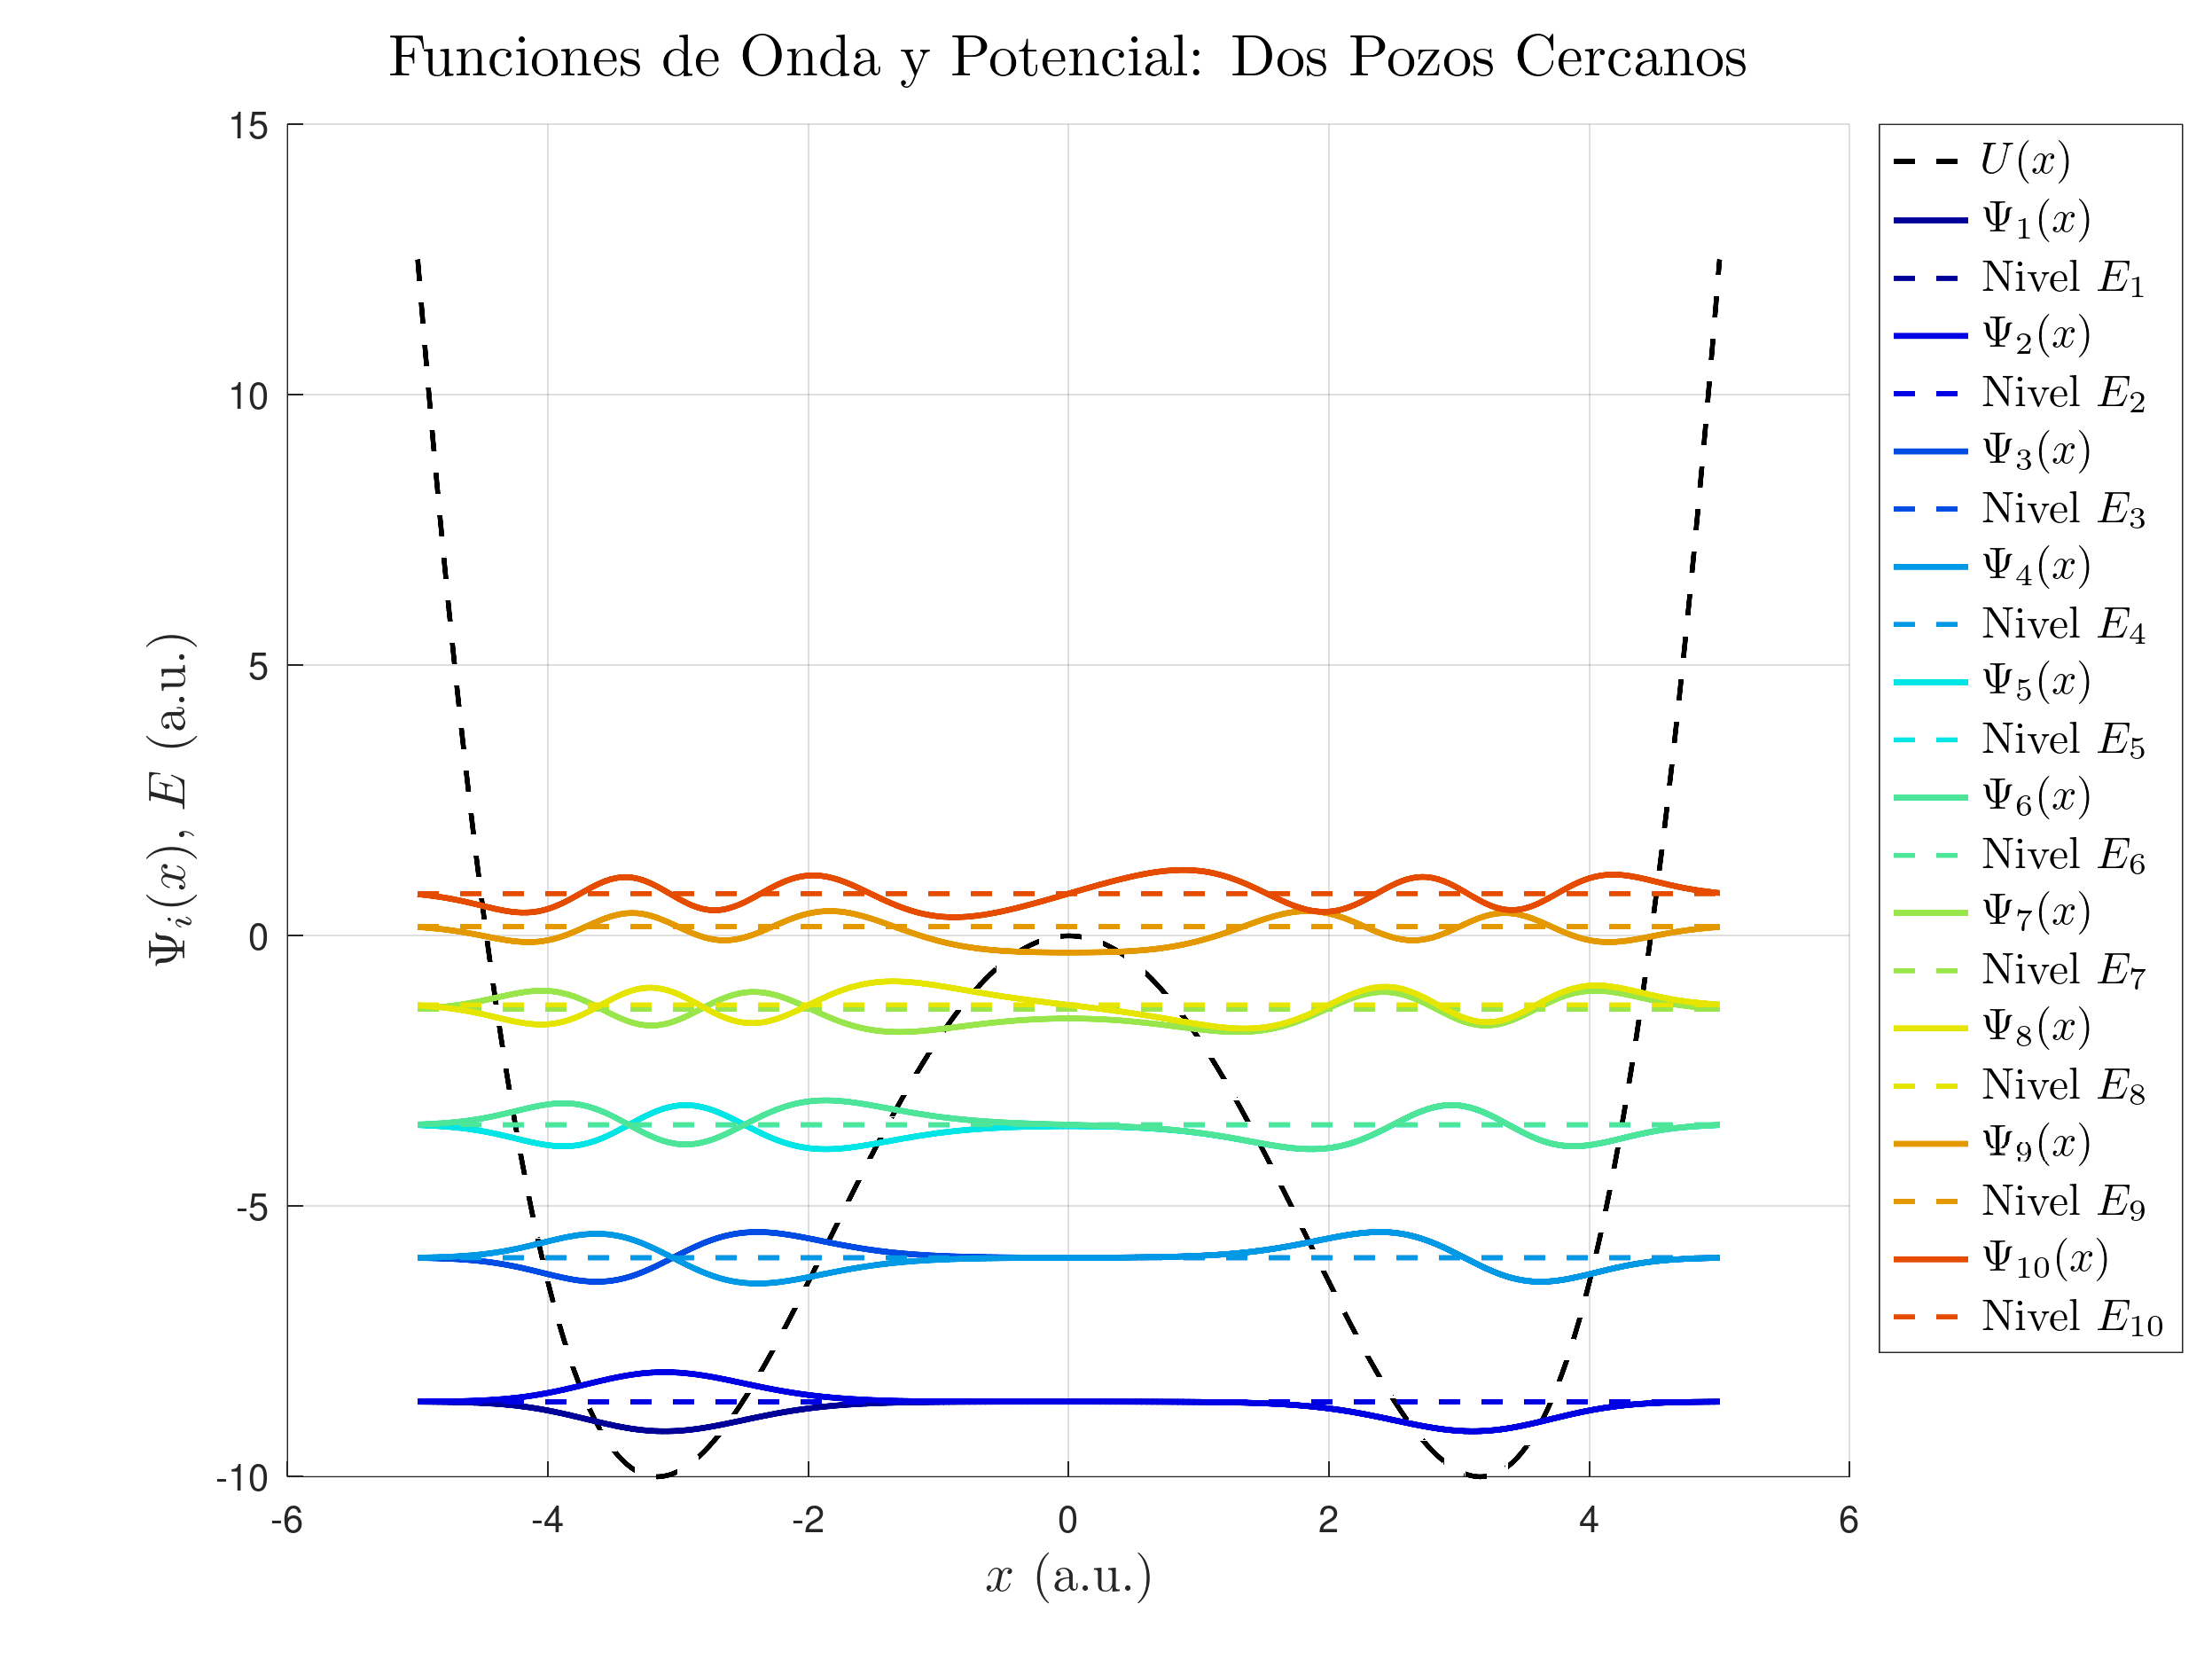
\includegraphics[width=0.9\textwidth]{img/Dos_Pozos_Cercanos_medium.png}
    \caption{Potencial de Dos Pozos Cercanos - Barrera baja}
    \label{fig:dos_pozos_cercanos_medium}
\end{figure}

\noindent
La Figura \ref{fig:dos_pozos_cercanos_medium} representa el potencial en un régimen con una barrera más baja que los niveles más altos de energía representados. Se evidencia que los estados acoplados se dan en los niveles más bajos, viendo claramente los estados simétrico y antisimétrico.

\begin{figure}[H]
    \centering
    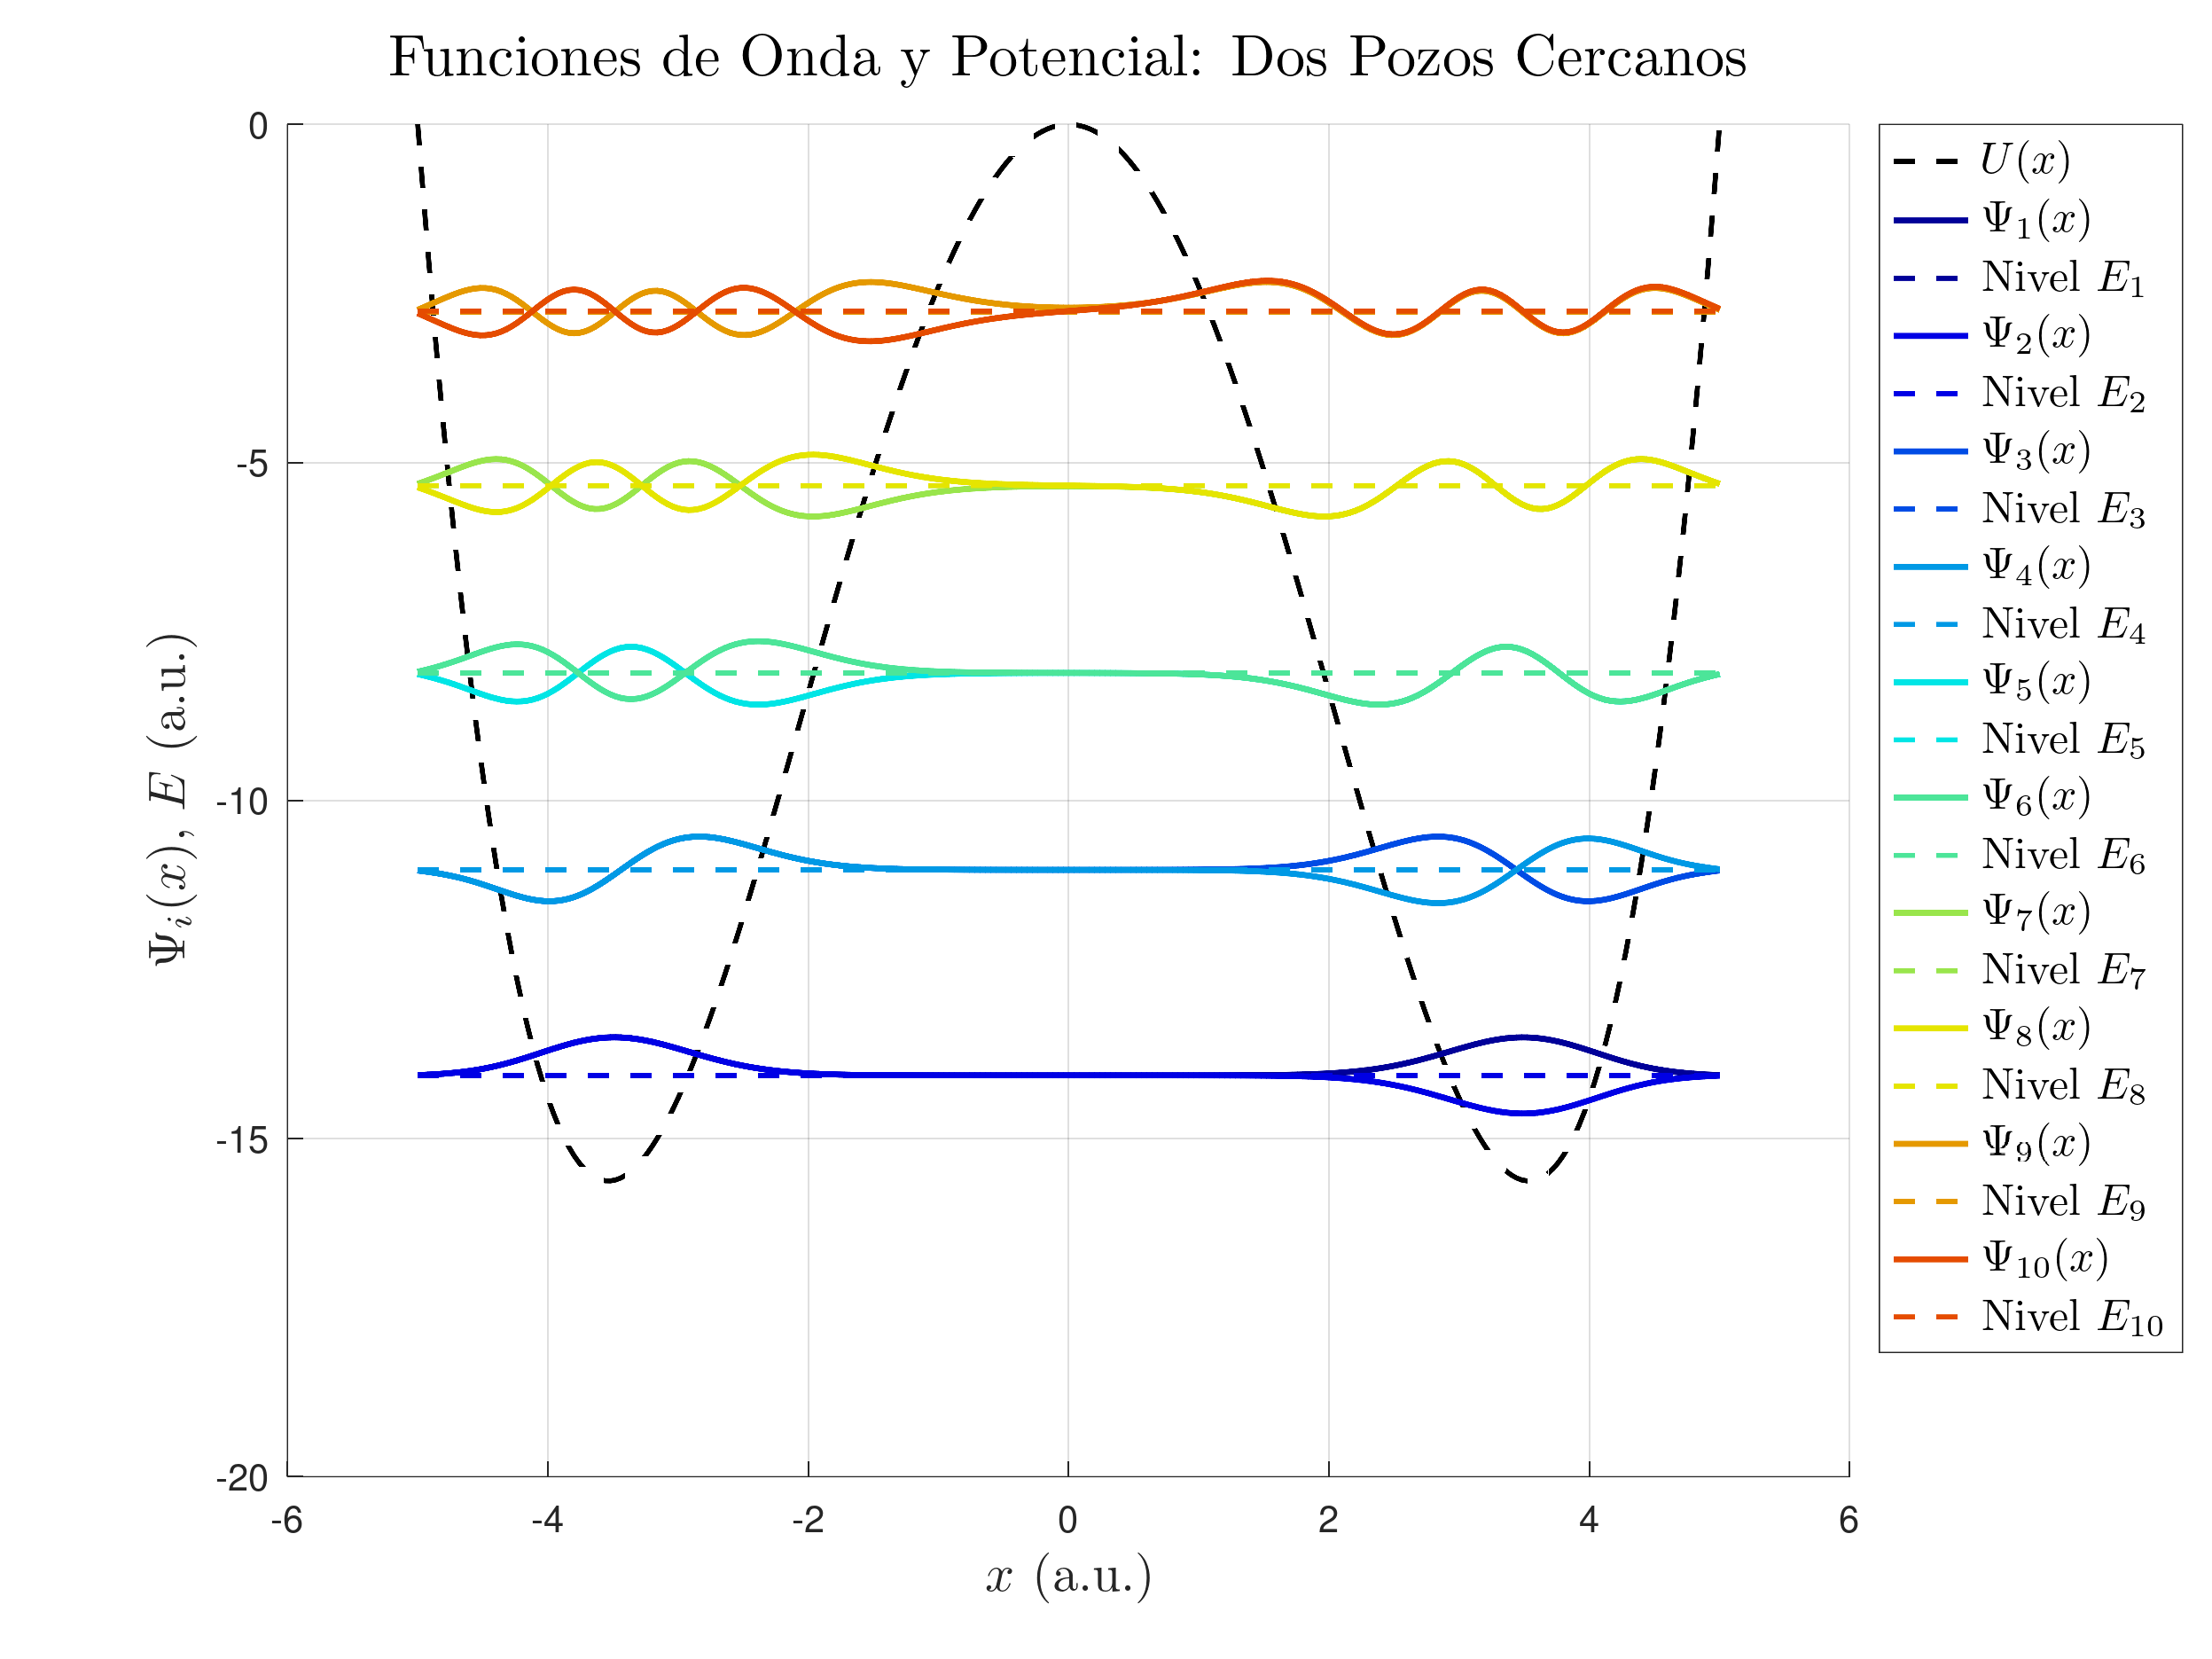
\includegraphics[width=0.9\textwidth]{img/Dos_Pozos_Cercanos_high.png}
    \caption{Potencial de Dos Pozos Cercanos - Barrera alta}
    \label{fig:dos_pozos_cercanos_high}
\end{figure}

\noindent
Finalmente, en la Figura \ref{fig:dos_pozos_cercanos_high} se ilustra el potencial en el régimen de una barrera más alta que el caso anterior. Las soluciones pueden ser aproximadas por dos osciladores armónicos en torno a los dos puntos de equilibrio estable, comprobamos que los pares de niveles simétrico y antisimétrico comparten nivel de energía y son prácticamente equidistantes con el resto de pares.

\subsubsection{Aplicaciones y Relevancia}

El potencial de dos pozos cercanos no solo es una herramienta teórica para entender conceptos fundamentales de la mecánica cuántica, sino que también tiene múltiples aplicaciones prácticas:

\subsubsection{Aplicaciones y Relevancia}

El potencial de dos pozos cercanos no solo es una herramienta teórica para entender conceptos fundamentales de la mecánica cuántica, sino que también tiene múltiples aplicaciones prácticas en diversas áreas de la física, la química y la tecnología avanzada. A continuación, se detallan algunas de las aplicaciones más destacadas:

\begin{itemize}
    \item \textbf{Qubits en Computación Cuántica}: 
    En la computación cuántica, los qubits son las unidades básicas de información cuántica. Los qubits superconductores, por ejemplo, a menudo se modelan como partículas en potenciales de dos pozos. En este contexto, los dos estados del qubit (\(|0\rangle\) y \(|1\rangle\)) corresponden a las posiciones de la partícula en cada pozo. Esta representación permite la implementación de operaciones cuánticas mediante la manipulación del potencial, facilitando la superposición y el entrelazamiento de estados, fundamentales para el procesamiento de información cuántica. Además, la coherencia cuántica entre los estados de los pozos es crucial para el correcto funcionamiento de los qubits, lo que requiere un control preciso sobre el acoplamiento y la barrera de potencial.
    
    \item \textbf{Moléculas Diatómicas}: 
    En química, el potencial de dos pozos cercanos es fundamental para describir la dinámica de las moléculas diatómicas. Estas moléculas, que consisten en dos átomos unidos por un enlace químico, presentan potenciales de energía que pueden tener múltiples configuraciones estables debido a diferentes estados de enlace. El modelo de dos pozos permite analizar cómo los átomos en una molécula diatómica pueden existir en diferentes estados de vibración y rotación, así como cómo pueden transitar entre estos estados mediante el efecto túnel cuántico. Esto es esencial para comprender procesos como la espectroscopía molecular, las reacciones químicas y las propiedades termodinámicas de gases diatómicos.
    
    \item \textbf{Fenómenos de Superconductividad y Superfluidez}: 
    El acoplamiento entre estados en potenciales de dos pozos es análogo a la formación de pares de Cooper en superconductores. En estos materiales, los electrones forman pares que se comportan como bosones y pueden moverse sin resistencia a través del material. Este fenómeno de acoplamiento es esencial para la explicación de la superconductividad y la superfluidez, y el modelo de dos pozos proporciona una base teórica para entender cómo estos pares interactúan y se acoplan en sistemas superconductores.
    
\end{itemize}

\subsubsection{Soluciones Cuánticas y Aproximaciones}

Resolver exactamente la ecuación de Schrödinger para el potencial de dos pozos cercanos es, en general, complejo y no siempre posible de manera analítica. Sin embargo, existen varias aproximaciones y métodos numéricos que permiten estudiar sus propiedades:

\begin{itemize}
    \item \textbf{Aproximación de Dos Niveles}: Como se mencionó anteriormente, esta aproximación simplifica el sistema considerando únicamente los dos estados fundamentales de cada pozo, facilitando el análisis de la dinámica cuántica y el acoplamiento entre estados.
    
    \item \textbf{Método de Perturbaciones}: Cuando el acoplamiento entre los pozos es débil, se puede tratar el término de acoplamiento como una perturbación y calcular las correcciones a los niveles de energía.
    
    \item \textbf{Métodos Numéricos}: Técnicas como la diagonalización matricial, el método de diferencias finitas y los métodos de elementos finitos permiten obtener soluciones aproximadas para la función de onda y los niveles de energía.
\end{itemize}

\subsubsection{Consideraciones Finales}

El estudio del potencial de dos pozos cercanos es esencial para comprender una amplia gama de fenómenos cuánticos donde la dualidad partícula-onda y el efecto túnel juegan roles cruciales. La capacidad de modelar y analizar sistemas con múltiples estados de equilibrio permite avanzar en áreas como la computación cuántica, la química teórica y la física de materiales. Además, el potencial de dos pozos sirve como un puente entre modelos simples y sistemas más complejos, proporcionando una base sólida para el desarrollo de teorías y aplicaciones avanzadas en la mecánica cuántica.

\subsection{Pozo Finito de Potencial}

El pozo finito de potencial es una aproximación más realista que el pozo infinito, ya que considera una profundidad limitada \( U_0 \) y una anchura \( 2L \). Se describe mediante la siguiente función de potencial:

\begin{equation}
    U(x) = \begin{cases} 
    -U_0 & \text{si } |x| < L \\ 
    0 & \text{si } |x| \geq L 
    \end{cases}
\end{equation}

A diferencia del pozo infinito, el pozo finito permite que las partículas tengan una pequeña probabilidad de escapar del pozo a través del efecto túnel, un fenómeno puramente cuántico que no ocurre en la descripción clásica.

\subsubsection{Soluciones de la Ecuación de Schrödinger}

Las soluciones de la ecuación de Schrödinger para el pozo finito incluyen tanto estados ligados (\( E < 0 \)) como estados no ligados (\( E > 0 \)). En los estados ligados, las funciones de onda están confinadas principalmente dentro del pozo pero tienen colas exponenciales que se extienden fuera de él, reflejando la probabilidad de túnel. Los niveles de energía no son equiespaciados y dependen de la profundidad \( U_0 \) y la anchura \( L \) del pozo. A mayor \( U_0 \) o \( L \), se incrementa el número de niveles de energía ligados.

\subsubsection{Efecto Túnel}

El efecto túnel es una característica distintiva del pozo finito, permitiendo que partículas con energía menor que \( U_0 \) atraviesen las barreras de potencial. Este fenómeno es fundamental en procesos como la emisión de electrones en diodos túnel y en reacciones nucleares de fisión.

\subsubsection{Sistemas Físicos Similares}

El pozo finito de potencial es útil para modelar diversos sistemas físicos, tales como:

\begin{itemize}
    \item \textbf{Pozos Cuánticos en Semiconductores}: Donde electrones o huecos están confinados en regiones de material con diferentes bandas de energía.
    \item \textbf{Nucleones en el Núcleo Atómico}: Modelando la interacción entre protones y neutrones dentro del núcleo.
    \item \textbf{Dispositivos Electrónicos}: Como diodos y transistores, donde el control del flujo de electrones a través de barreras de potencial es esencial.
\end{itemize}

\begin{figure}[H]
    \centering
    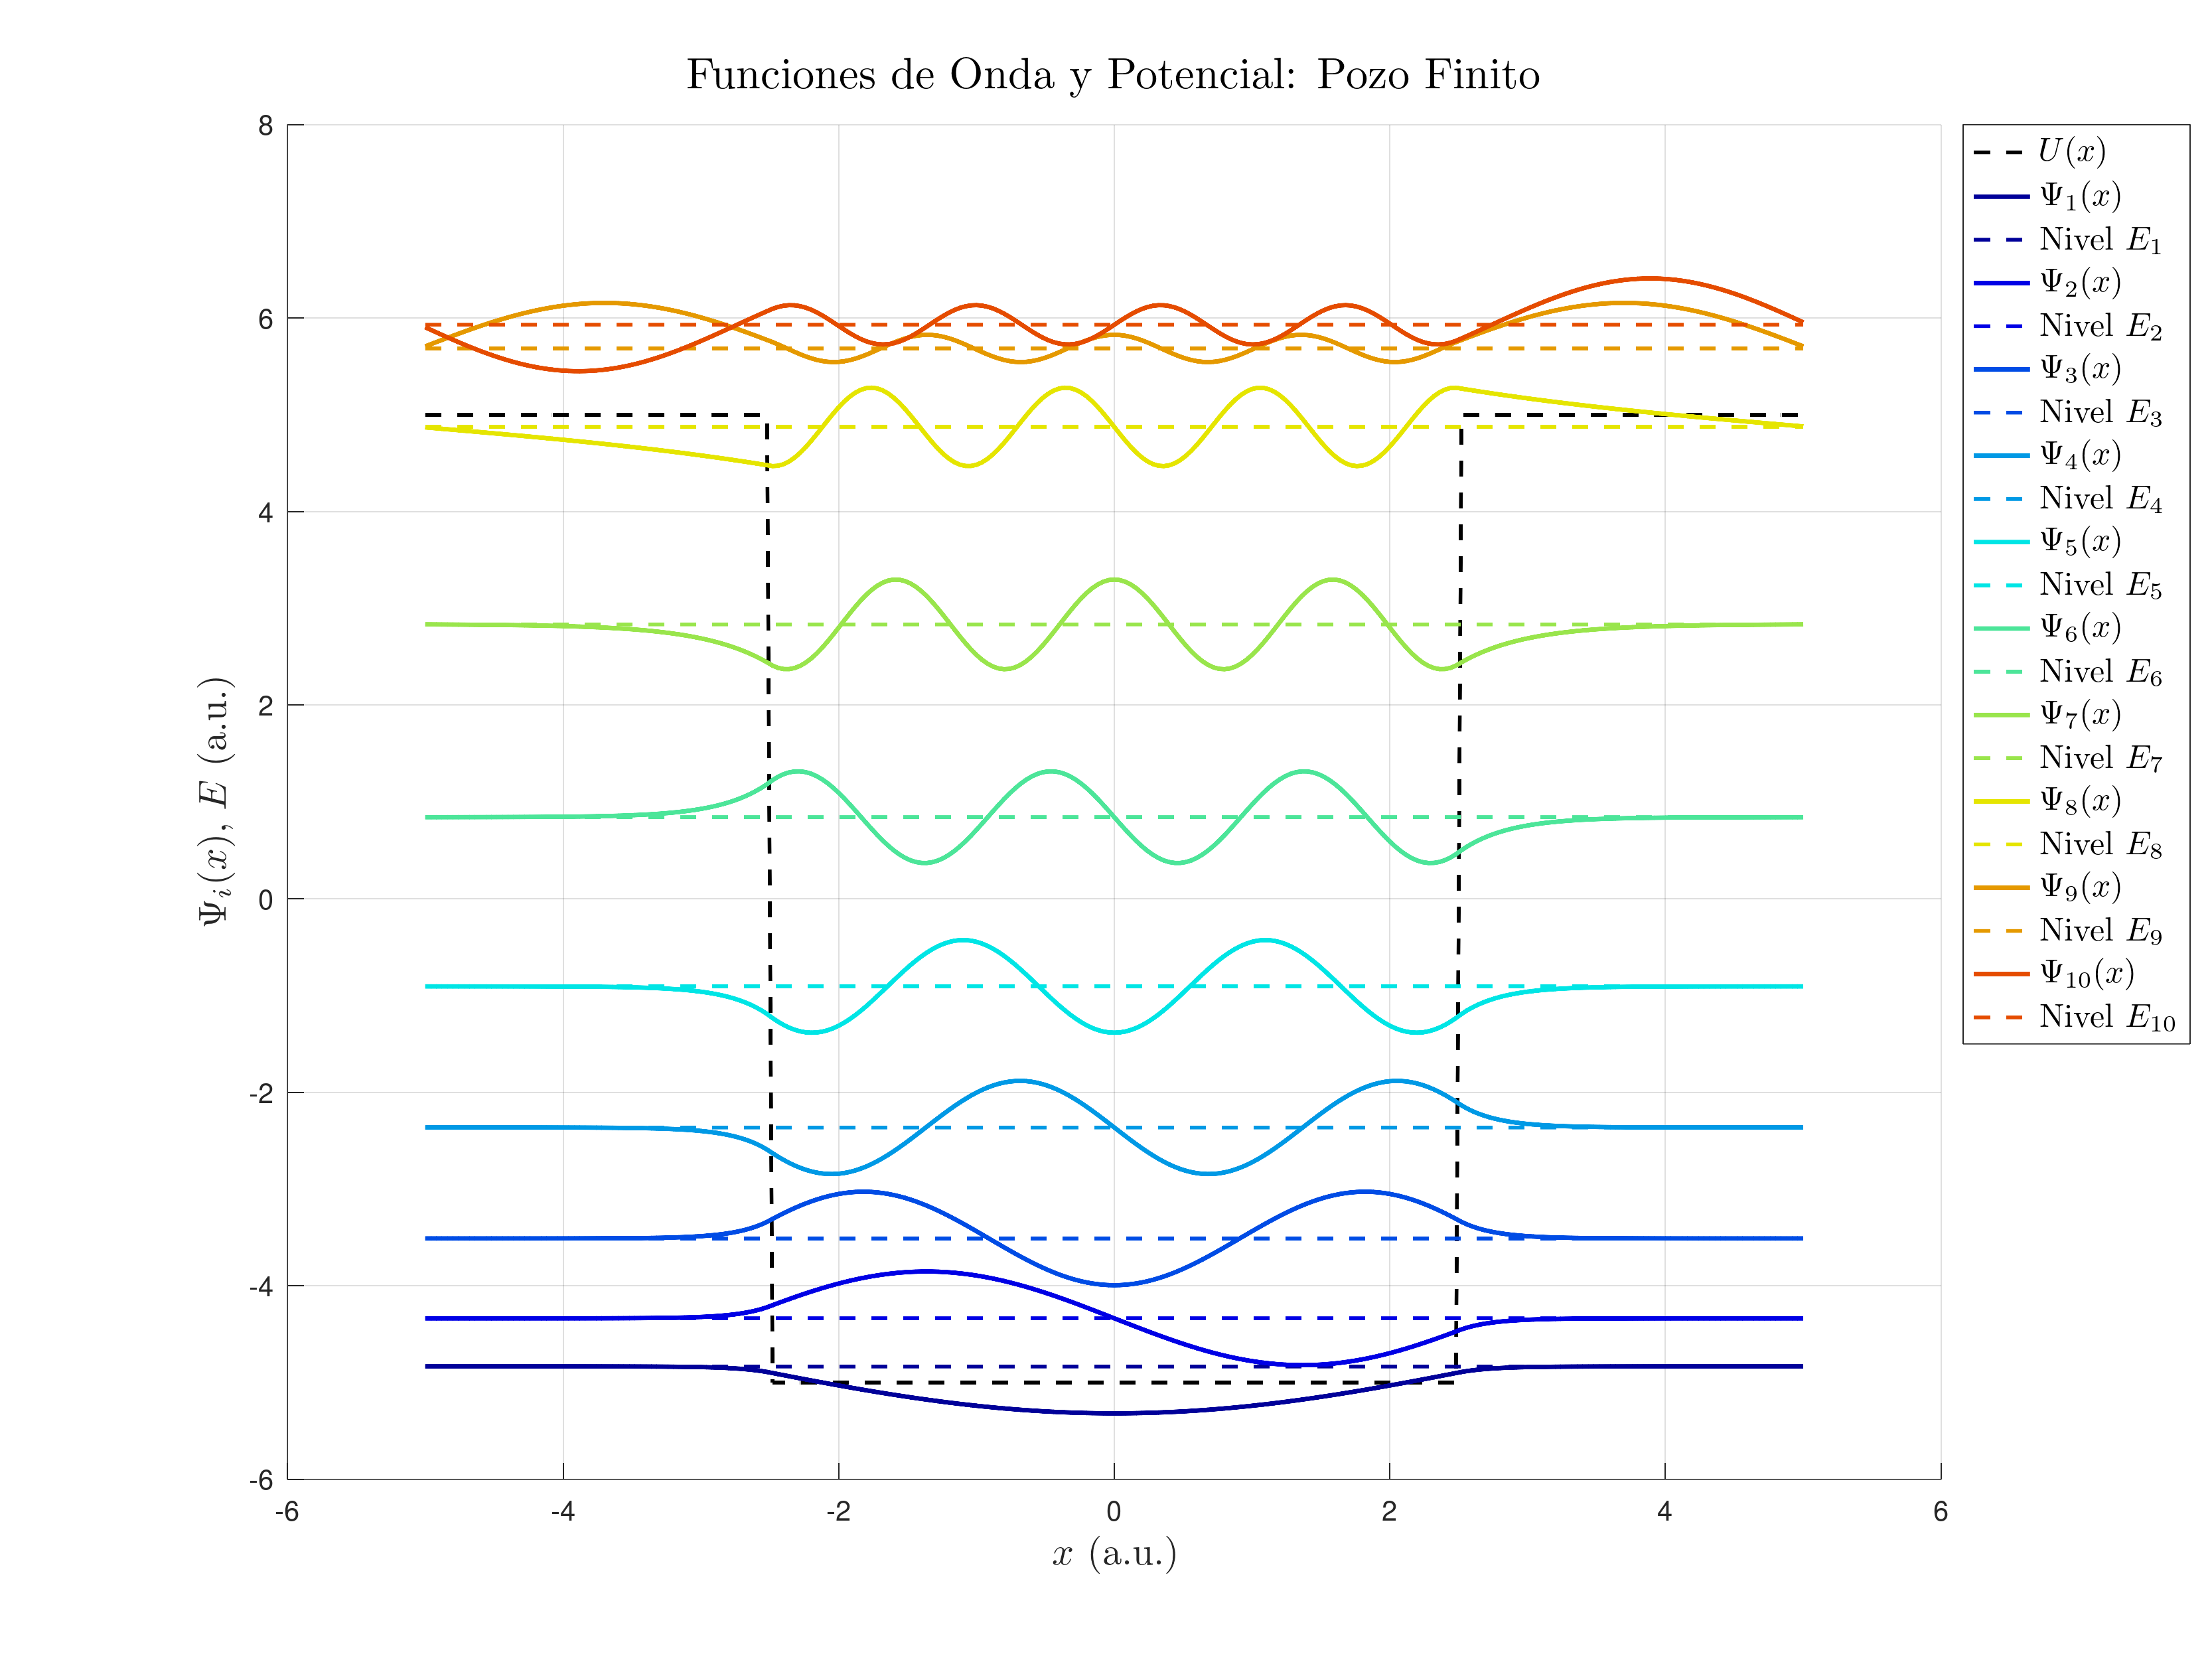
\includegraphics[width=0.9\textwidth]{img/Pozo_Finito.png}
    \caption{Pozo Finito de Potencial con Niveles de Energía y Funciones de Onda Correspondientes}
    \label{fig:pozo_finito}
\end{figure}

\noindent
En la Figura \ref{fig:pozo_finito} se observa el perfil del pozo finito de potencial \( U(x) \) junto con varios niveles de energía \( E_n \) y sus correspondientes funciones de onda \( \psi_n(x) \). Los niveles de energía ligados están por debajo de \( U(x) = 5 \) y muestran funciones de onda localizadas dentro del pozo con colas que se extienden fuera de él, indicando la posibilidad de túnel. A diferencia del pozo infinito, las funciones de onda no son nulas fuera del pozo, lo que permite la existencia de estados de resonancia y una distribución de niveles de energía más realista.

\subsection{Potencial de Kronig-Penney}

El modelo de Kronig-Penney introduce la periodicidad en el estudio de los potenciales en la mecánica cuántica, siendo fundamental para la comprensión de las propiedades electrónicas de los sólidos cristalinos. Este modelo simplificado representa un potencial periódico compuesto por una sucesión infinita de pozos de potencial representados por funciones delta de Dirac. La expresión matemática del potencial es:

\begin{equation}
    U(x) = \sum_{n=-\infty}^{\infty} V_0 \delta(x - na)
\end{equation}

donde \( V_0 \) es la profundidad de cada pozo de potencial, \( a \) es la distancia entre los pozos, y \( n \) es un entero que recorre todos los pozos en el espacio. Este potencial modela una cadena unidimensional de átomos idénticos, capturando la periodicidad que caracteriza a los cristales sólidos.

\subsubsection{Formulación del Modelo}

El modelo de Kronig-Penney se basa en la resolución de la ecuación de Schrödinger independiente del tiempo para un electrón en un potencial periódico. Aplicando el teorema de Bloch, las soluciones de la ecuación de Schrödinger en este potencial toman la forma de funciones de Bloch:

\begin{equation}
    \psi_k(x) = e^{ikx} u_k(x)
\end{equation}

donde \( u_k(x) \) es una función periódica con la misma periodicidad que el potencial, y \( k \) es el número de onda. La periodicidad del potencial lleva a la formación de bandas de energía y huecos de banda, fenómenos cruciales para entender la conductividad eléctrica en materiales sólidos.

\subsubsection{Formación de Bandas de Energía}

La periodicidad del potencial de Kronig-Penney conduce a la aparición de bandas de energía \( E(k) \) donde los electrones pueden existir y a huecos de banda donde no es posible encontrar estados permitidos para los electrones. Estos huecos de banda son responsables de las propiedades semiconductoras y aislantes de los materiales.

La relación de dispersión para este modelo se obtiene resolviendo la ecuación de Schrödinger con el potencial periódico, lo que resulta en una ecuación que relaciona \( E \) y \( k \). La solución muestra que, para ciertas condiciones de \( V_0 \) y \( a \), se forman bandas de energía separadas por huecos.

\begin{figure}[H]
    \centering
    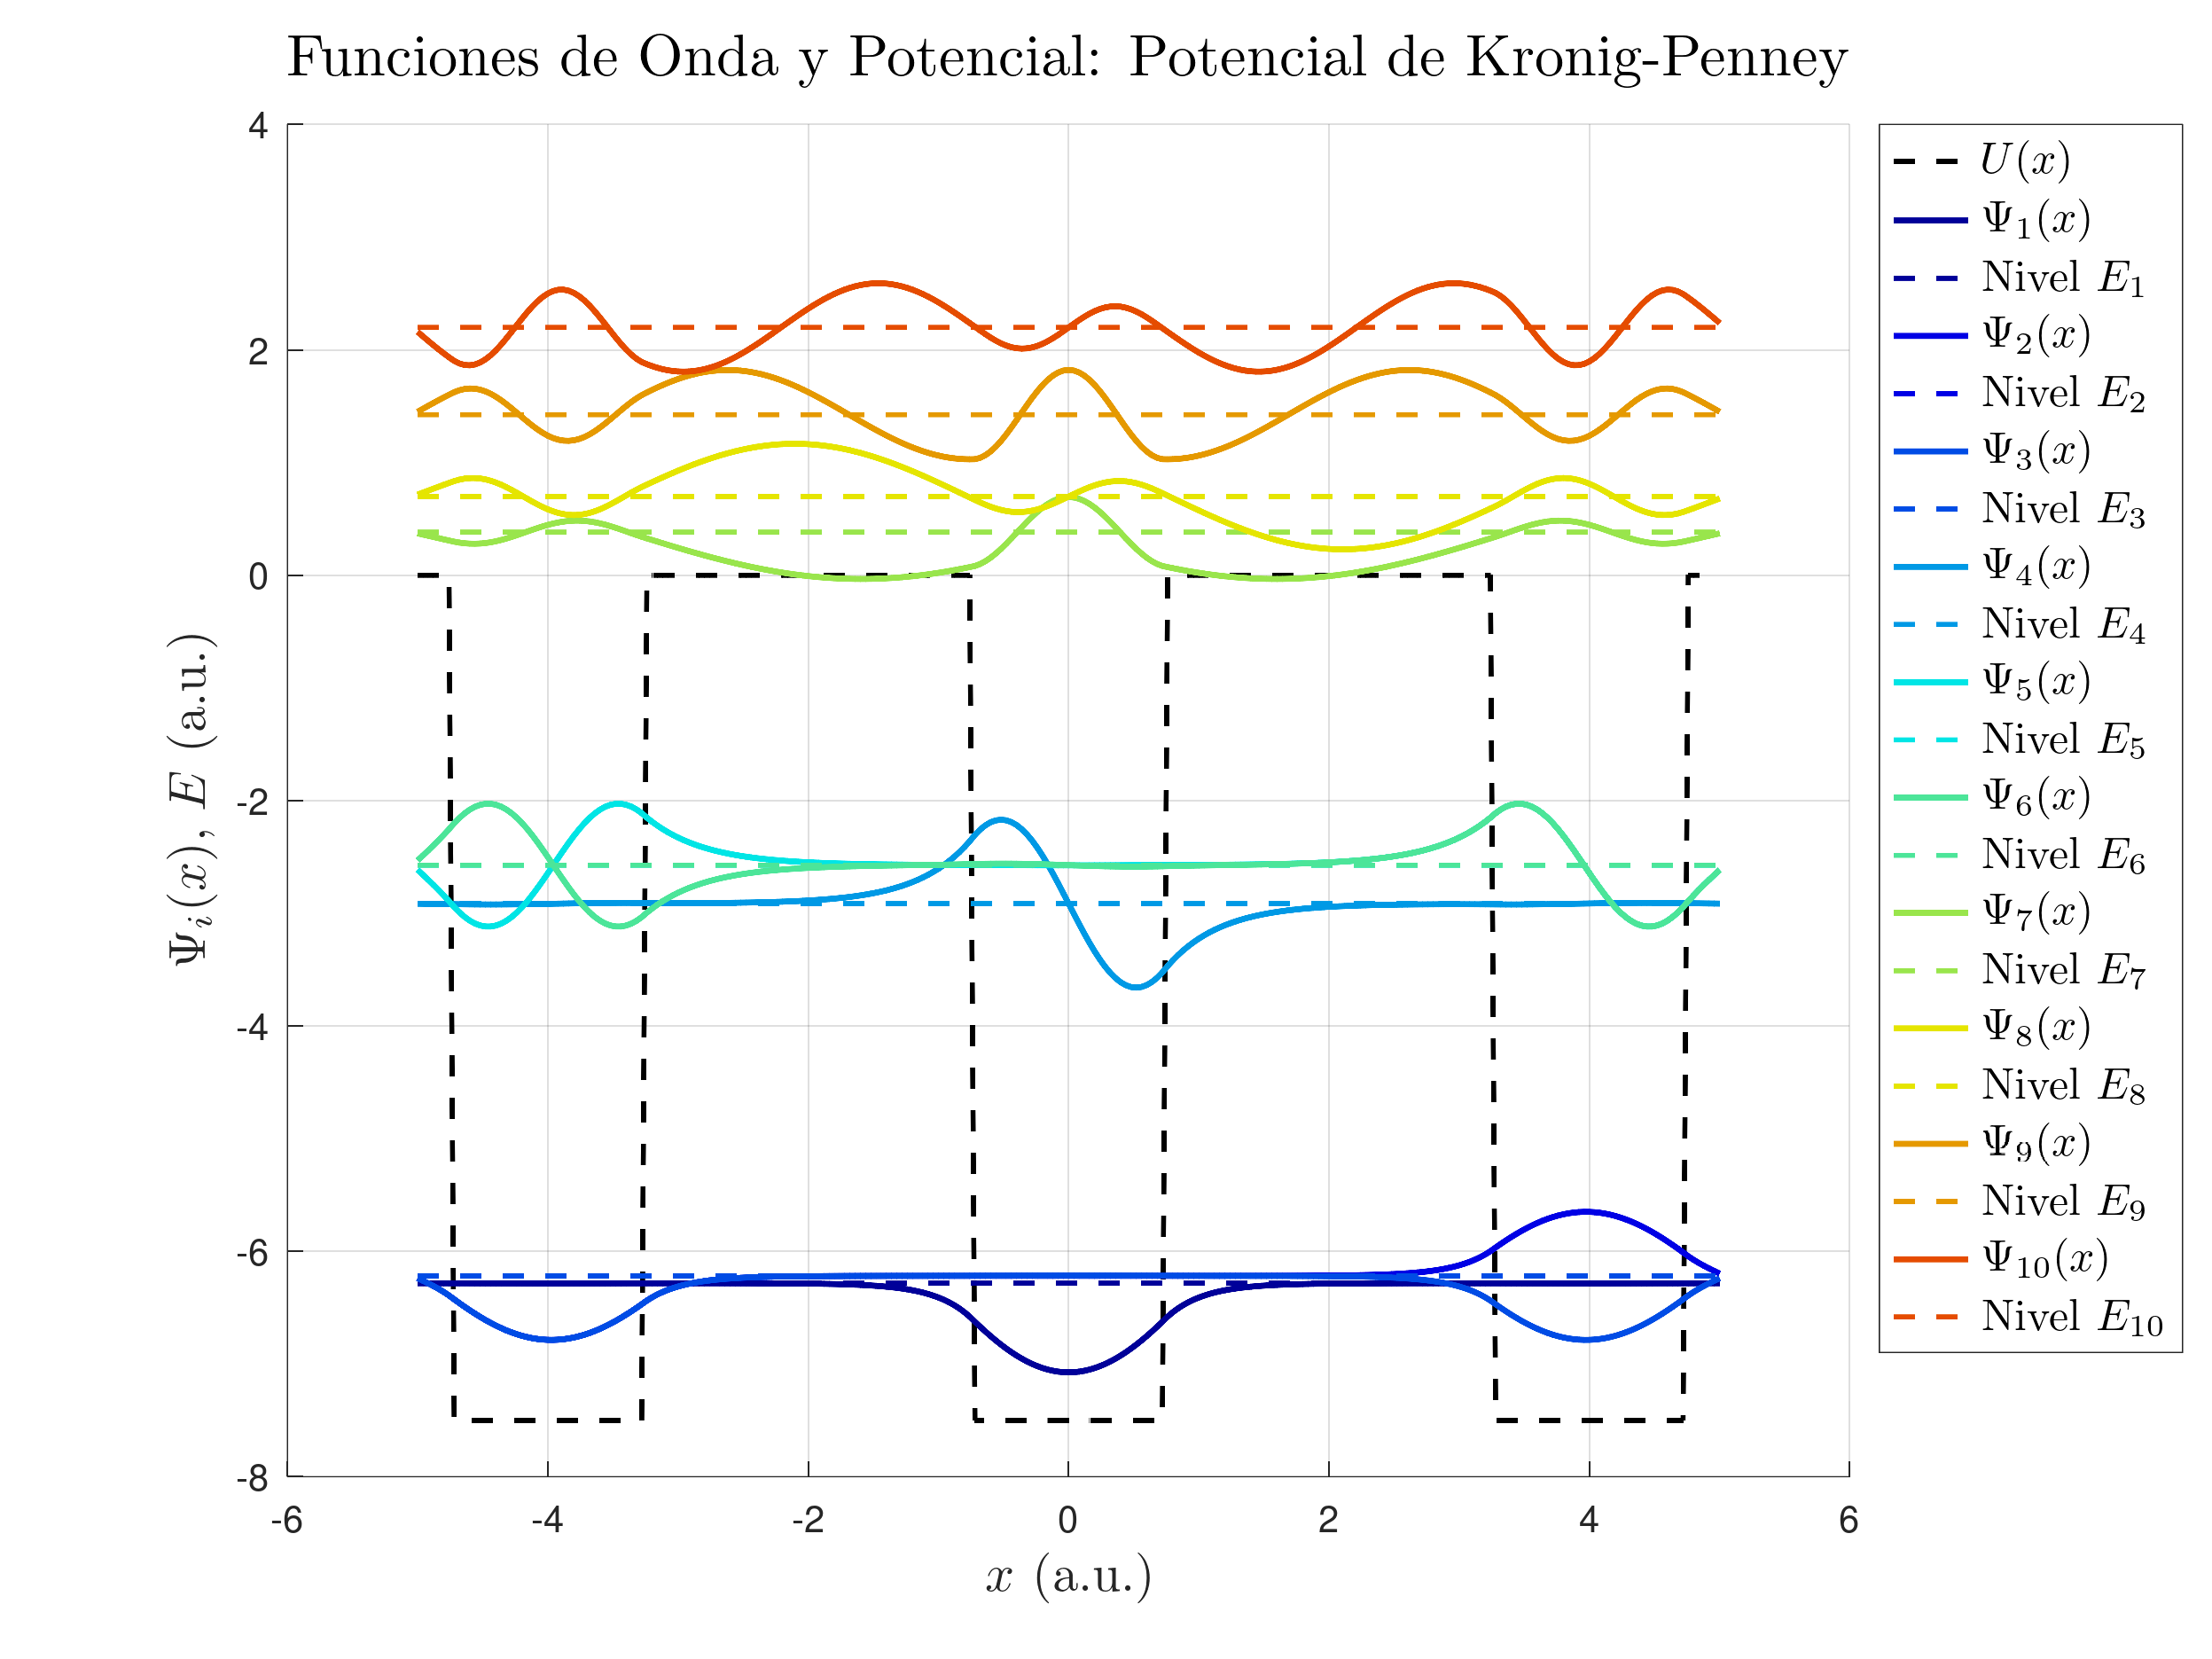
\includegraphics[width=0.9\textwidth]{img/Potencial_de_Kronig-Penney_low.png}
    \caption{Potencial de Kronig-Penney - Bajo número de pozos}
    \label{fig:kronig_penney_low}
\end{figure}

En la figura \ref{fig:kronig_penney_low} se muestra el potencial de Kronig-Penney con tres de pozos. En esta configuración observamos la formación de 5 niveles no ligados y otros 5 ligados divididos en 2 bandas.

\begin{figure}[H]
    \centering
    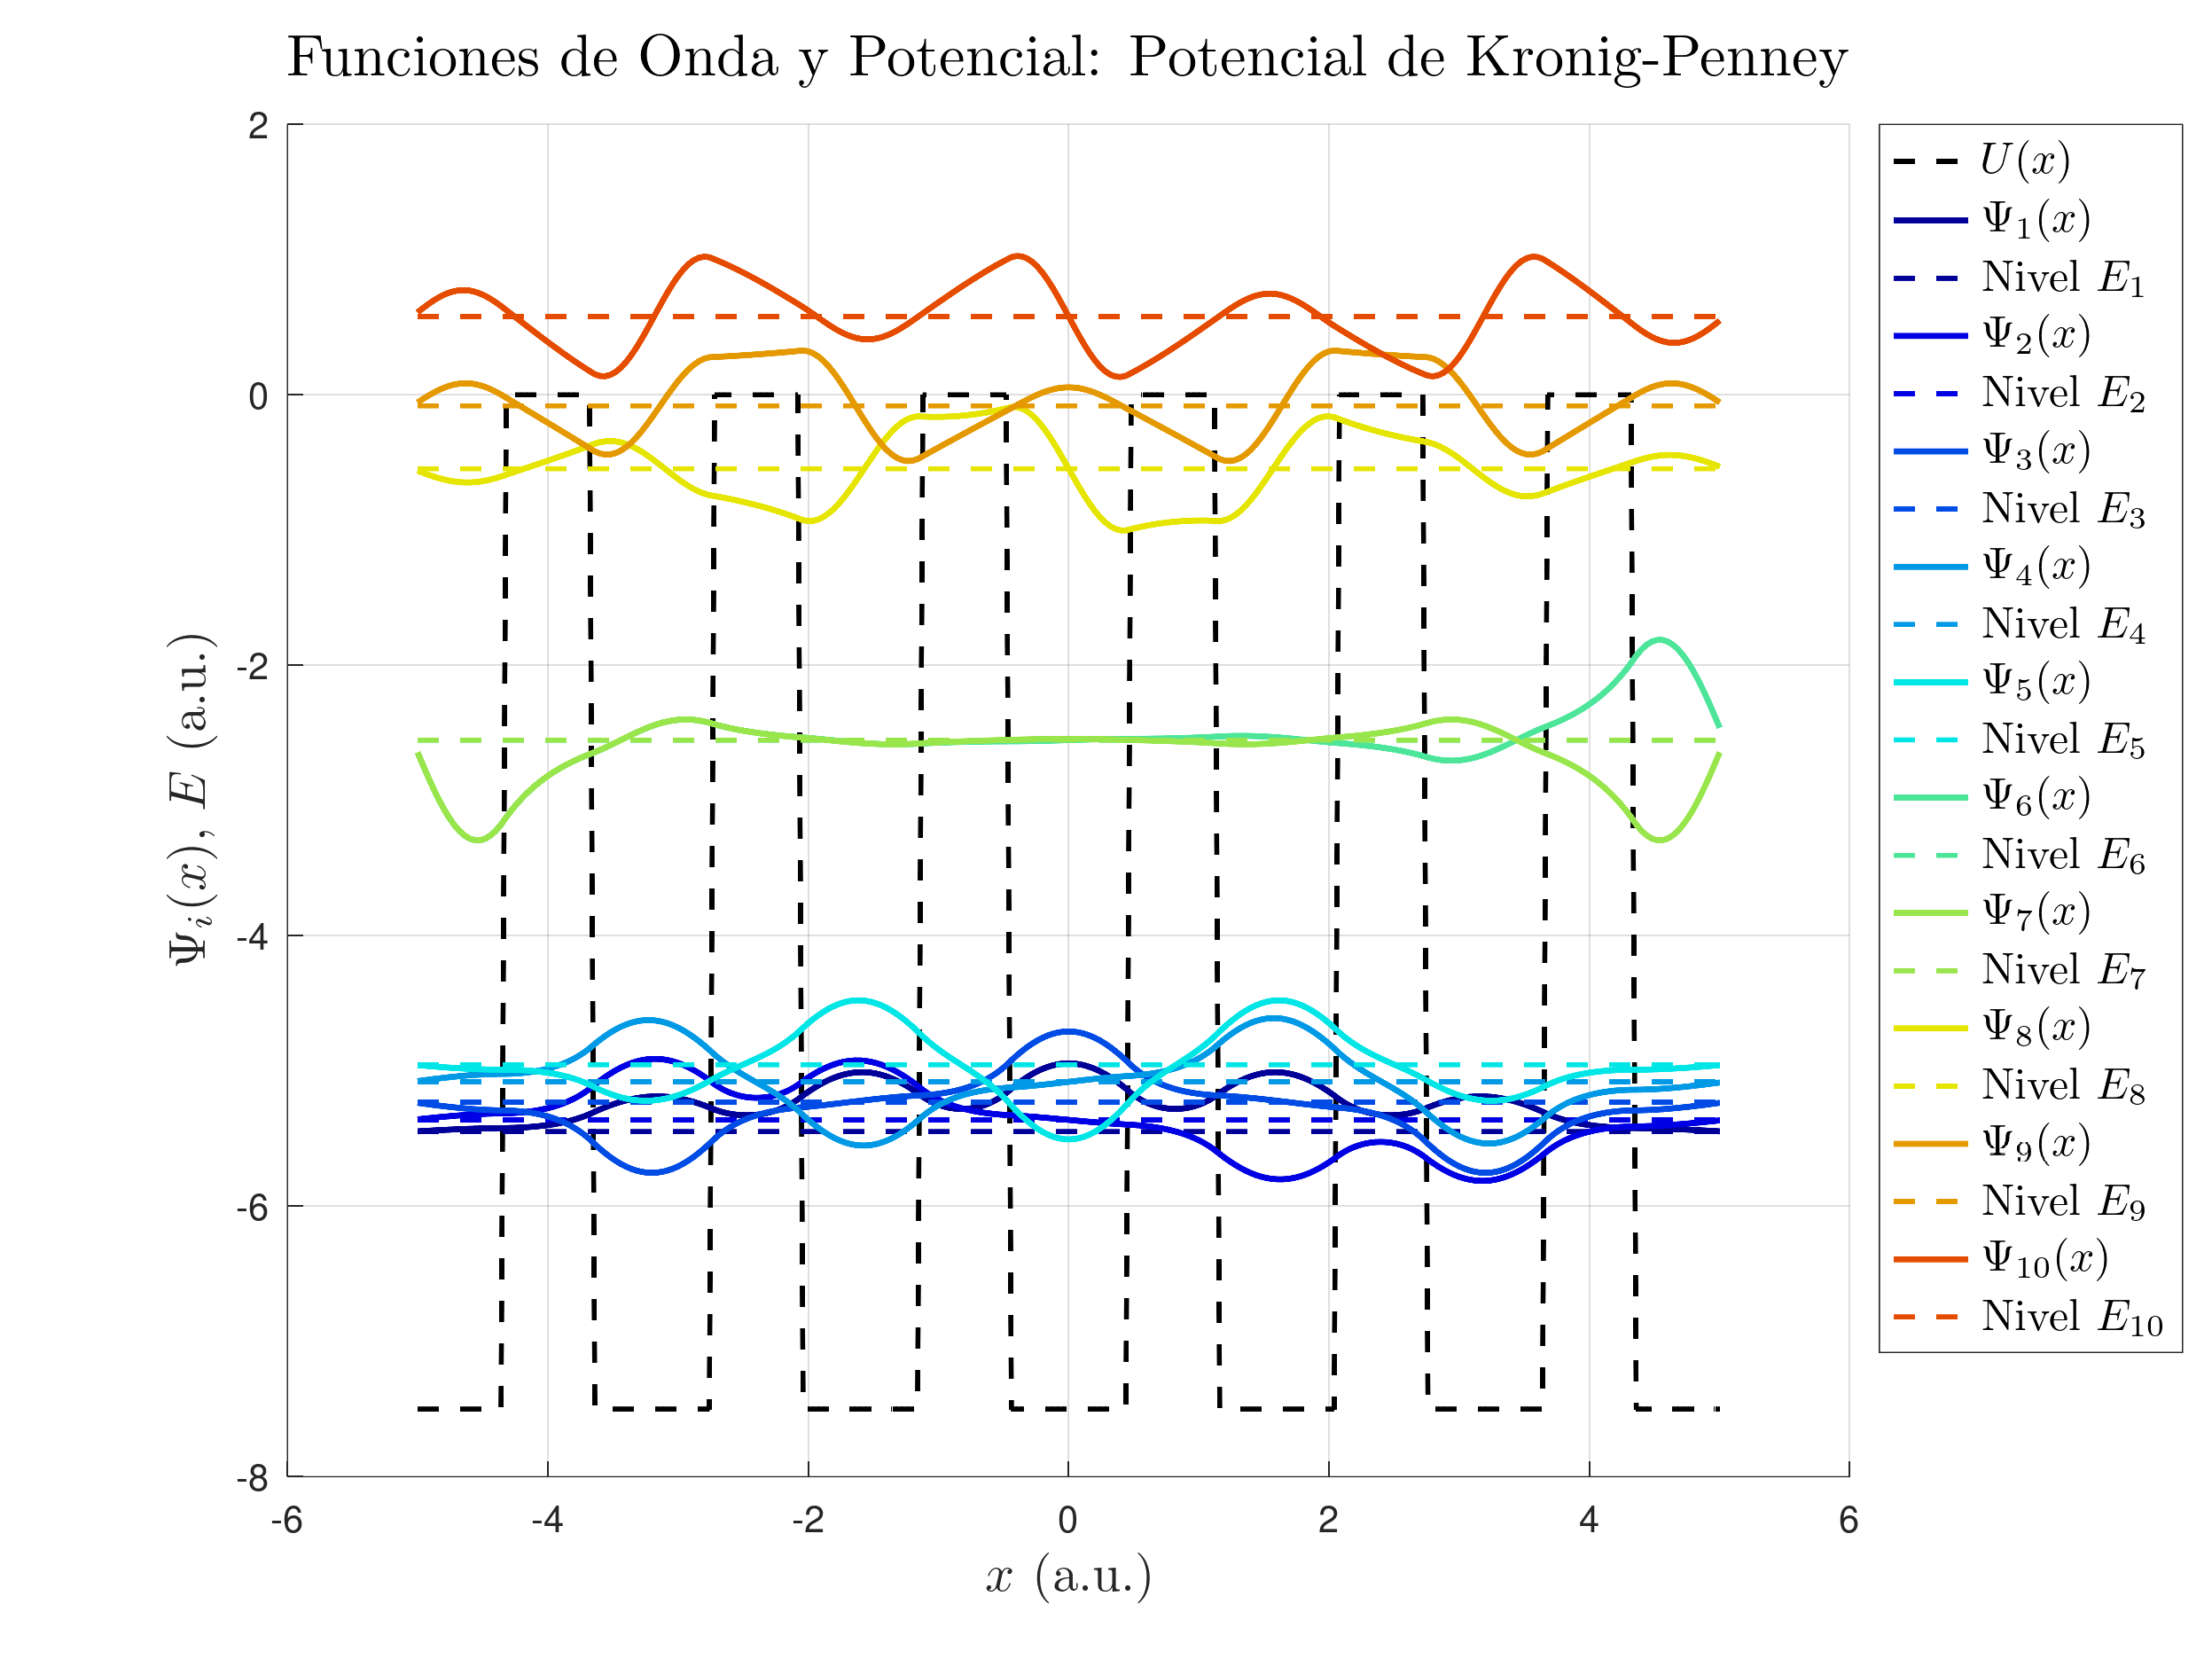
\includegraphics[width=0.9\textwidth]{img/Potencial_de_Kronig-Penney_medium.png}
    \caption{Potencial de Kronig-Penney - Número medio de pozos}
    \label{fig:kronig_penney_medium}
\end{figure}
En la figura \ref{fig:kronig_penney_medium} se muestra el potencial de Kronig-Penney con cinco de pozos. Observamos igualmente la formación de bandas y huecos y en los niveles de energía superiores, la formación de estados no ligados.

\begin{figure}[H]
    \centering
    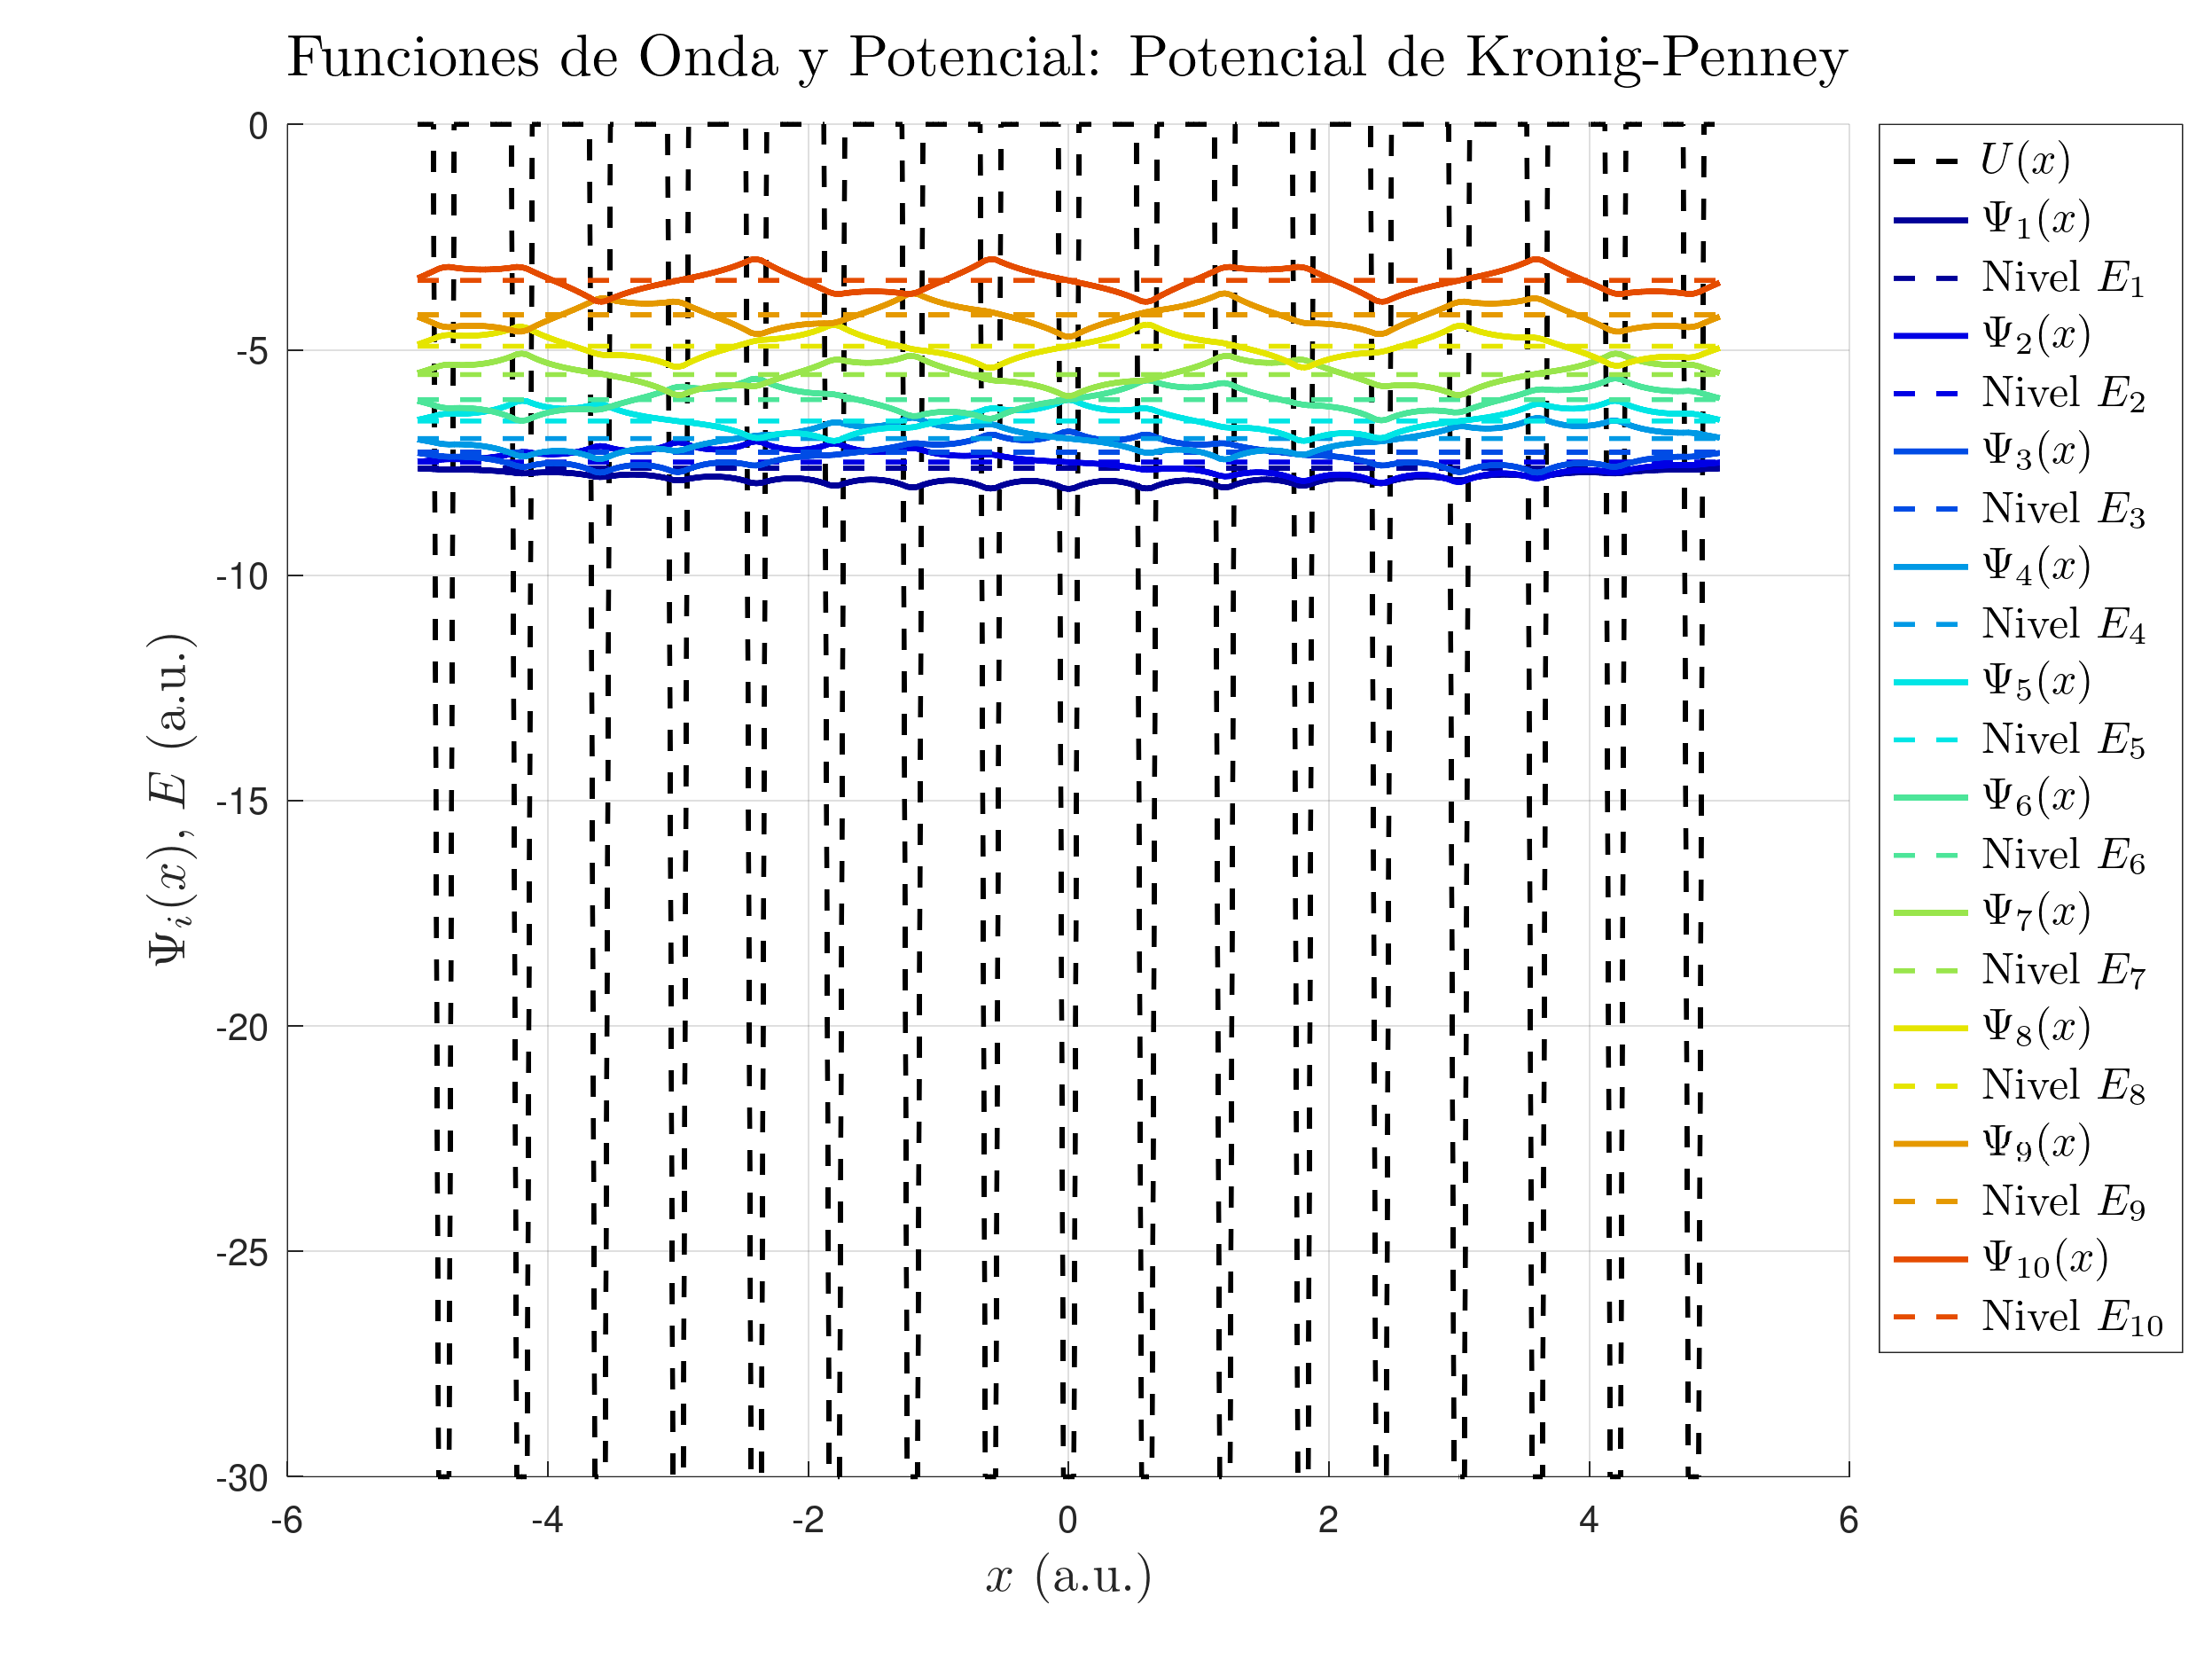
\includegraphics[width=0.9\textwidth]{img/Potencial_de_Kronig-Penney_high.png}
    \caption{Potencial de Kronig-Penney - Alto número de pozos}
    \label{fig:kronig_penney_high}
\end{figure}

Finalmente, la figura \ref{fig:kronig_penney_high} ilustra el potencial de Kronig-Penney con un alto número de pozos, simulando una estructura cristalina extensa. En este caso las bandas aparecen más cercanas entre sí. Observamos para los niveles de energía mas altos, la presencia de "picos", mientras que para niveles más bajos las funciones de onda resultan más suaves.

\subsubsection{Importancia del Modelo de Kronig-Penney}

El modelo de Kronig-Penney es fundamental en la física del estado sólido por varias razones:

\begin{enumerate}
    \item \textbf{Formación de Bandas de Energía}: Proporciona una comprensión clara y matemática de cómo se forman las bandas de energía y los huecos de banda debido a la periodicidad del potencial.
    
    \item \textbf{Teoría de Bloch}: Sirve como un ejemplo ilustrativo para la aplicación del teorema de Bloch, que establece que las soluciones de la ecuación de Schrödinger en un potencial periódico pueden ser expresadas como funciones de Bloch.
    
    \item \textbf{Propiedades Electrónicas}: Ayuda a explicar las diferencias entre conductores, semiconductores y aislantes a partir de la estructura de bandas.
    
    \item \textbf{Base para Modelos Más Complejos}: Forma la base para modelos más complejos en la teoría de bandas, permitiendo la inclusión de efectos como el entrelazamiento de bandas, interacciones electrón-electrón y defectos cristalinos.
\end{enumerate}

\subsubsection{Limitaciones del Modelo}

A pesar de su utilidad, el modelo de Kronig-Penney presenta ciertas limitaciones:

\begin{itemize}
    \item \textbf{Simplificación del Potencial}: Utiliza potenciales delta, que son idealizaciones matemáticas. En la realidad, los potenciales de los átomos en un cristal tienen una forma más compleja.
    
    \item \textbf{Dimensionalidad Unidimensional}: El modelo original es unidimensional, lo que limita su aplicabilidad directa a sistemas tridimensionales reales.
    
    \item \textbf{Ignora Interacciones Electrón-Electrón}: No considera las interacciones entre los electrones, lo que es crucial para una descripción más completa de los materiales.
\end{itemize}

A pesar de estas limitaciones, el modelo de Kronig-Penney sigue siendo una herramienta educativa y teórica valiosa para entender los fundamentos de la estructura de bandas en sólidos.

\subsubsection{Extensiones y Aplicaciones Avanzadas}

El modelo de Kronig-Penney ha sido extendido y modificado para abordar situaciones más realistas, tales como:

\begin{itemize}
    \item \textbf{Potenciales Periódicos con Diferentes Formas}: Se han estudiado potenciales periódicos con formas más realistas que las delta de Dirac para mejorar la precisión del modelo.
    
    \item \textbf{Incorporación de Defectos}: Se han introducido defectos en la periodicidad para estudiar efectos como los estados localizados y las impurezas.
    
    \item \textbf{Aplicaciones en Nanotecnología}: Adaptaciones del modelo han sido utilizadas para analizar propiedades electrónicas en estructuras nanoscópicas como nanocables y nanocristales.
\end{itemize}

\section{Conclusiones}
En este trabajo hemos explorado diversos tipos de pozos de potencial, desde los más simples hasta algo más complejos, y sus aplicaciones en distintos contextos físicos. Cada modelo aporta una perspectiva única sobre cómo las partículas cuánticas interactúan con campos potenciales, permitiendo la comprensión de fenómenos como el efecto túnel, la formación de bandas de energía y la estabilidad de enlaces moleculares. La inclusión de múltiples figuras para cada tipo de potencial facilita la visualización de estos conceptos, reflejando la complejidad y las características distintivas de cada sistema estudiado.

\section*{Comentarios}
La realización de esta tarea práctica me ha permitido profundizar en el uso de métodos numéricos para resolver ecuaciones diferenciales en mecánica cuántica. He aprendido a implementar un algoritmo como composición de distintos métodos numéricos y a representarlos correctamente. He entendido mejor los problemas de pozos de potencial, desde una perspectiva más computacional. He investigado sobre distintas aplicaciones de los modelos que se han expuesto, creando muy distintos potenciales (varios de los cuales al final no aparecen en el informe). Además, he mejorado mis habilidades en la redacción de informes científicos y en el manejo de \LaTeX.

\begin{thebibliography}{9}

\bibitem{ref1}
García, P., Alvarellos, J. E., \& García, J. J. (2012). \textit{Física Cuántica I}. UNED.

\bibitem{ref2}
Feynman, R. P., Leighton, R. B., \& Sands, M. (2011). \textit{The Feynman Lectures on Physics}. Basic Books.

\bibitem{ref3}
Maslov, D. L. (2012). \textit{Dirac-Kronig-Penney model}. \url{http://www.phys.ufl.edu/~maslov/phz6426/phz6426_dkp.pdf}

\bibitem{ref4}
Feynman, R. P., Leighton, R. B., \& Sands, M. (2010). \textit{The Feynman Lectures on Physics: Volume III}. \url{https://www.feynmanlectures.caltech.edu/III_toc.html}

\end{thebibliography}

\end{document}
